%!TEX program = xelatex
% Note: this template must be compiled with XeLaTeX rather than PDFLaTeX
% due to the custom fonts used. The line above should ensure this happens
% automatically, but if it doesn't, your LaTeX editor should have a simple toggle
% to switch to using XeLaTeX.

\documentclass[
  aspectratio=169, % Uncomment to use an aspect ratio of 16:9 (160 mm by 90 mm)
  %aspectratio=43, % Uncomment to use an aspect ratio of 4:3 (128mm by 96mm)
  t, % Top align all slide content by default
  onlytextwidth, % Typeset content in columns at text width
  10pt, % Default font size, use 10pt for the 16:9 aspect ratio and 8pt for the 4:3 aspect ratio
]{beamer}

\usepackage{../../ImperialTheme/beamer/beamerthemeImperial} % Use the Imperial theme
\usepackage{xcolor}

\definecolor{tabpurple}{RGB}{148, 103, 189}
\definecolor{tabcyan}{RGB}{23, 190, 207}
\definecolor{tabred}{RGB}{214, 39, 40}

\def\imagefolder{../../ImperialTheme/beamer/Images}
\def\Rey{\text{Re}}
\title{Re analysis} % Presentation title to appear on the title slide and left footers

\subtitle{} % Presentation subtitle to appear on the title slide

\author{Víctor Ballester} % Author name(s) to appear on the title slide

\date{\today} % Presentation date to appear on the title slide and right footers

\begin{document}

\begingroup
\setbeamercolor{background canvas}{bg=ICLLightGrey} % Slide background color
\setbeamercolor{title page title}{fg=ICLBlue} % Title text color
\setbeamercolor{title page subtitle}{fg=ICLBlue} % Subtitle text color
\setbeamercolor{author}{fg=ICLBlue} % Author(s) text color
\setbeamercolor{date}{fg=ICLBlue} % Date text color
\setbeamertemplate{title page}[logo]{\imagefolder/ICL_Logo_Blue.pdf} % Imperial logo color, use 'ICL_Logo_White.pdf' for white and 'ICL_Logo_Blue.pdf' for blue
\frame[plain, s]{\titlepage} % Output the title page with no footer ('plain') and vertically distributed text ('s')
\endgroup

\begin{frame}
	\frametitle{Summary of results (Re = 1000)}
	\begin{figure}[ht]
		\centering
		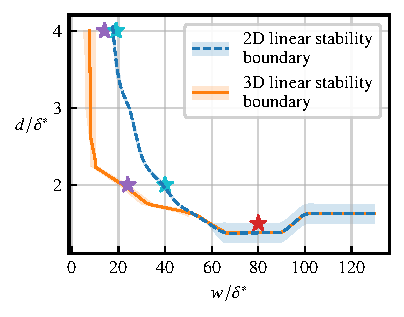
\includegraphics[width=10cm]{Images/3d2dStabilityCurveRe1000.pdf}
	\end{figure}
\end{frame}
\begin{frame}
	\frametitle{Case {\color{tabpurple}\Large\ding{72}}}
	\begin{columns}[T] % [T] ensures correct vertical alignment
		\begin{column}{0.495\linewidth} % left column
			\begin{figure}[ht]
				\centering
				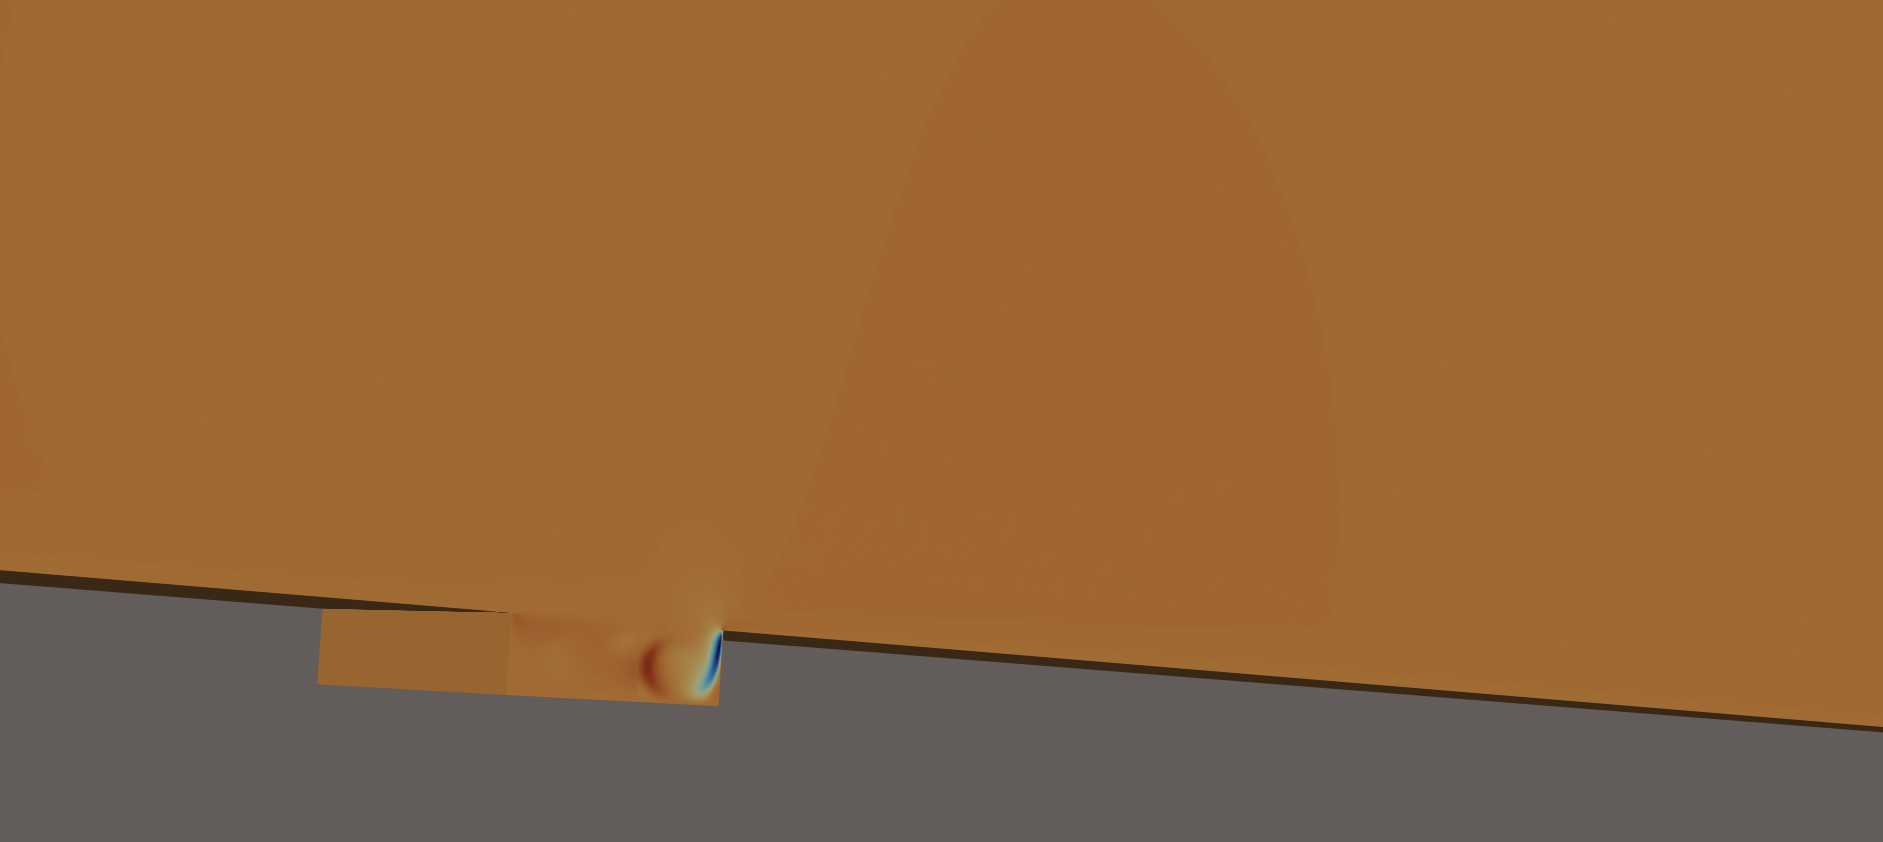
\includegraphics[width=\linewidth]{Images/3dmodestable2d.png}
			\end{figure}
			Full velocity $v$ field (very similar to the base state)
		\end{column}
		\begin{column}{0.495\linewidth} % left column
			\begin{figure}[ht]
				\centering
				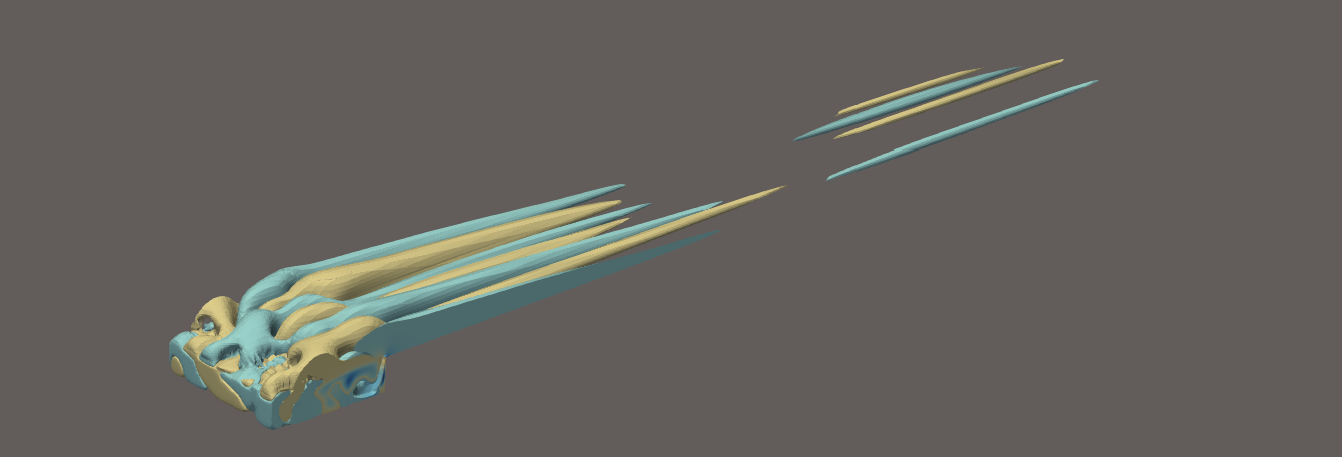
\includegraphics[width=\linewidth]{Images/3dmodestable2disovolumes.png}
			\end{figure}
			Perturbation $v$ field after being evolved with the nonlinear operator
		\end{column}
	\end{columns}
\end{frame}
\begin{frame}
	\frametitle{Case {\color{tabcyan}\Large\ding{72}}}
	\vspace{-1cm}
	\begin{columns}[T] % [T] ensures correct vertical alignment
		\begin{column}{0.45\linewidth} % left column
			\begin{figure}[ht]
				\centering
				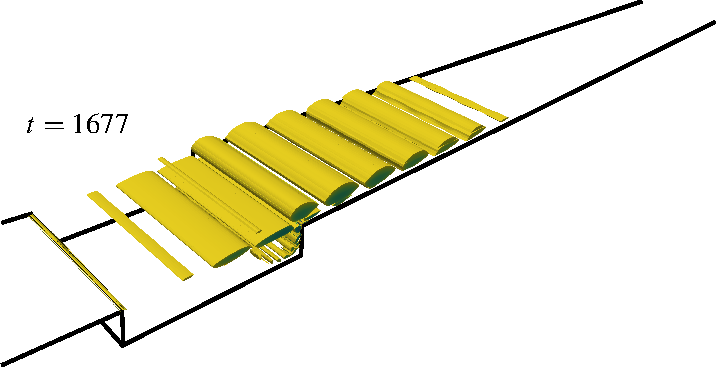
\includegraphics[width=\linewidth]{../../Images/3dTransParaview/pdfs/d4w19_3d_L2crit_10.pdf}
			\end{figure}
		\end{column}\hfill
		\begin{column}{0.45\linewidth} % left column
			\begin{figure}[ht]
				\centering
				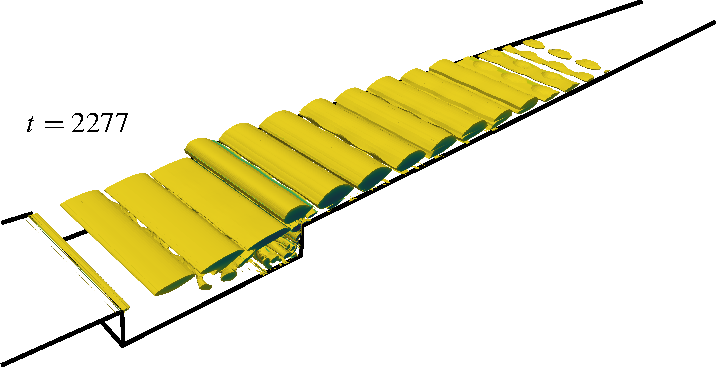
\includegraphics[width=\linewidth]{../../Images/3dTransParaview/pdfs/d4w19_3d_L2crit_12.pdf}
			\end{figure}
		\end{column}
	\end{columns}
	\vspace{-2cm}
\begin{columns}[T] % [T] ensures correct vertical alignment
		\begin{column}{0.45\linewidth} % left column
			\begin{figure}[ht]
				\centering
				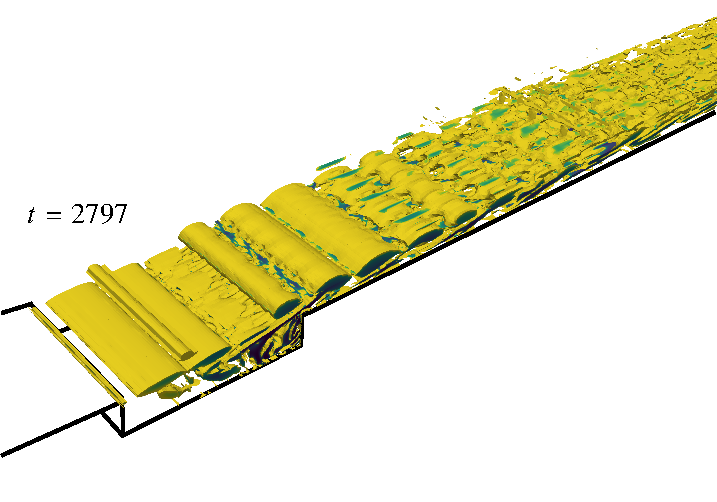
\includegraphics[width=\linewidth]{../../Images/3dTransParaview/pdfs/d4w19_3d_L2crit_14_big.pdf}
			\end{figure}
			\vspace{-0.5cm}
			Transition through secondary instability (floquet analysis)
		\end{column}\hfill
		\begin{column}{0.45\linewidth} % left column
			\begin{figure}[ht]
				\centering
				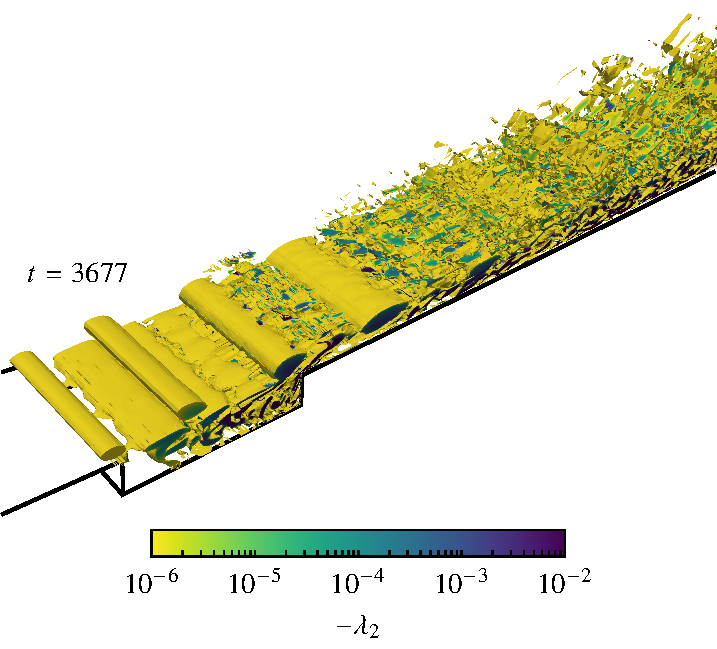
\includegraphics[width=\linewidth]{../../Images/3dTransParaview/pdfs/d4w19_3d_L2crit_17_big.pdf}
			\end{figure}
		\end{column}
	\end{columns}
\end{frame}
\begin{frame}
	\frametitle{Case {\color{tabcyan}\Large\ding{72}} - floquet mode}
	\begin{figure}[ht]
	  \centering
	  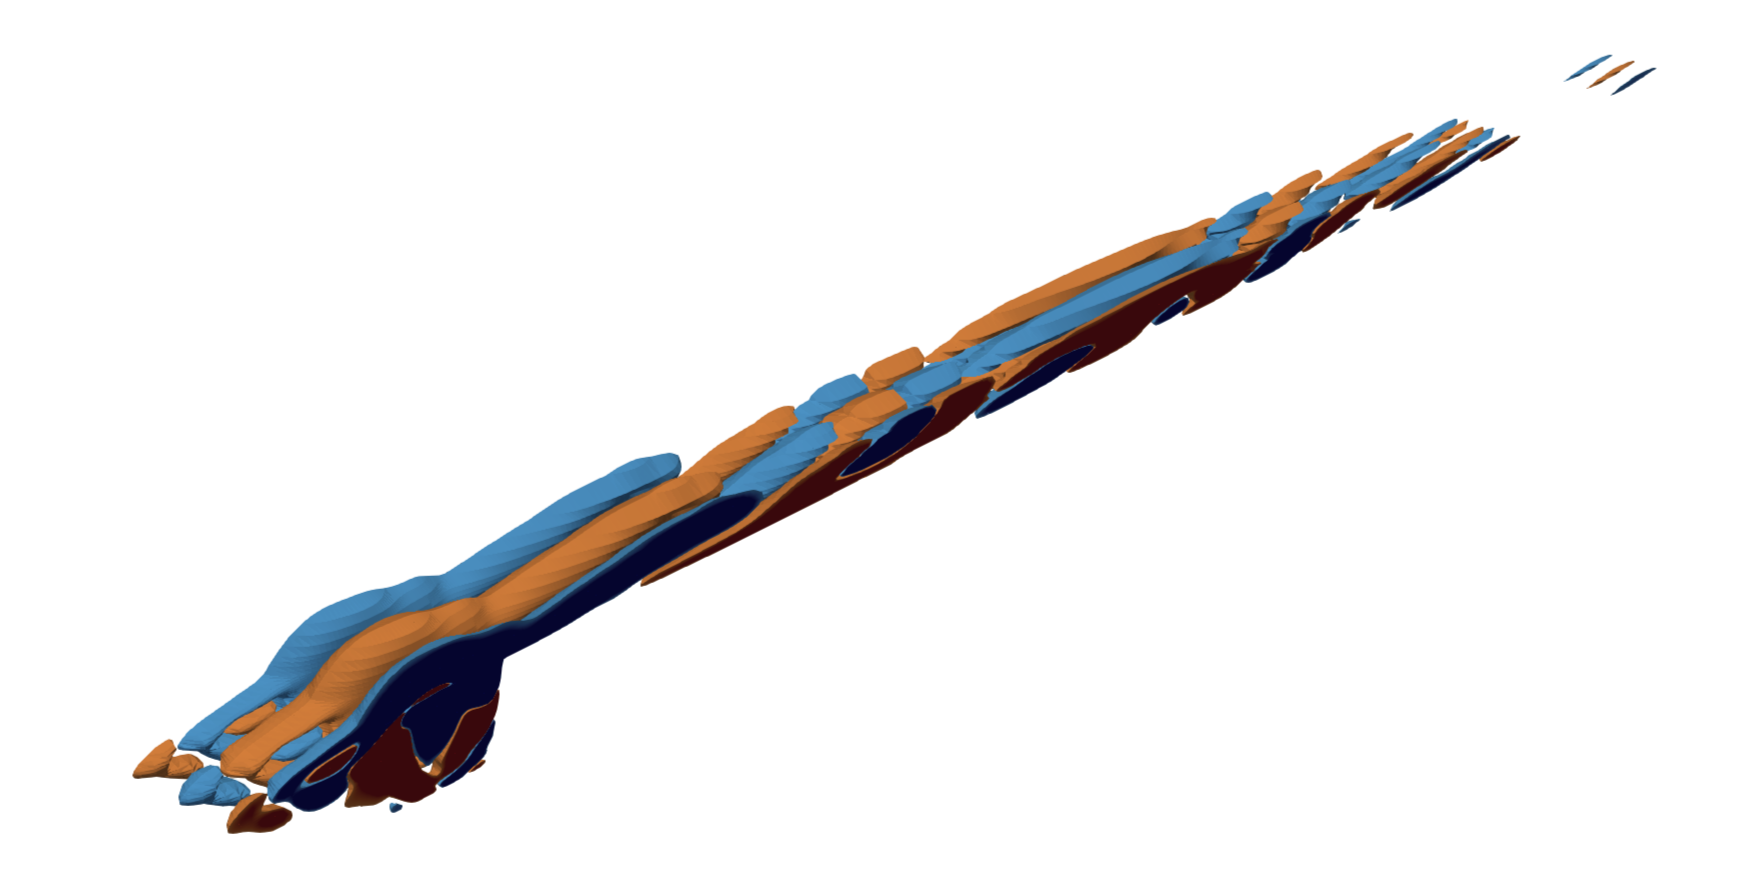
\includegraphics[width=\textwidth]{Images/floquetmode.png}
	\end{figure}
  
\end{frame}
\begin{frame}
	\frametitle{Case {\color{tabcyan}\Large\ding{72}}}
	About the appreance of the 2d mode first. Two diagnostics that I am currently doing:
	\begin{itemize}
	  \item First is run the direct solver with the 3d perturbation and the full set of modes (instead of just only one) to see if that modifies the growth rate of the whole 3d mode.
	  \item I have the feeling that any small noise trigger quickly the 2d mode, and I coarsen the mesh (maybe slightly to much) and that is why the 2d mode might appear first.
	\end{itemize}
\end{frame}
\begin{frame}
	\frametitle{Transition in case {\color{tabred}\Large\ding{72}}}
	Frequency of the most unstable 2d mode for this cavity is $\omega \approx 0.099$, which lies inside the unstable region of the neutral stability curve.
\begin{figure}[ht]
			\centering
			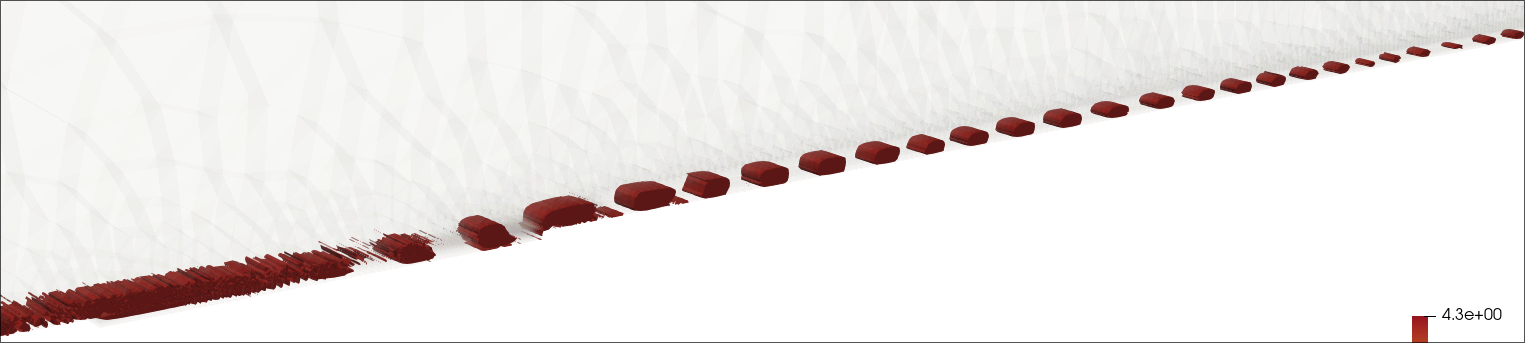
\includegraphics[width=\textwidth]{Images/d1.5w80_trans1.png}
		\end{figure}
\end{frame}
\begin{frame}
	\frametitle{Transition in case {\color{tabred}\Large\ding{72}}}
\begin{figure}[ht]
			\centering
			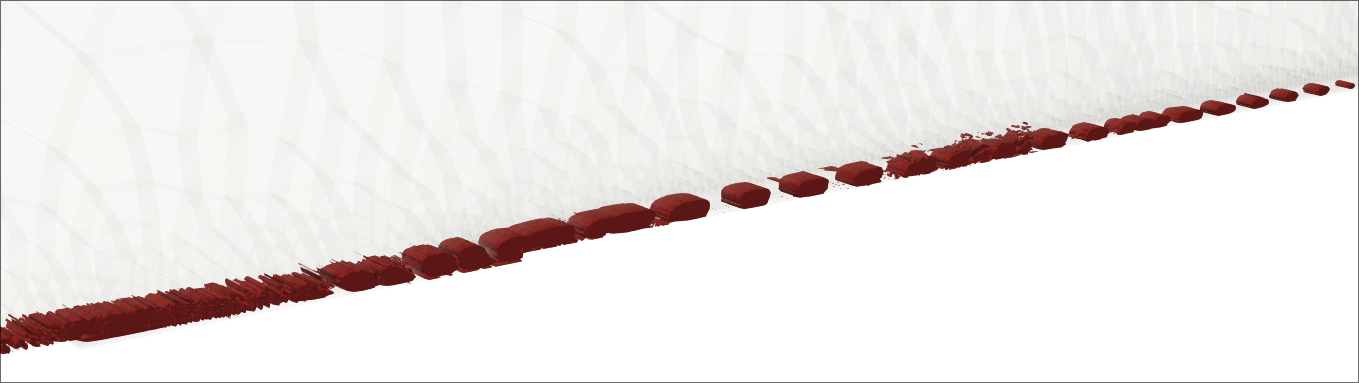
\includegraphics[width=\textwidth]{Images/d1.5w80_trans2.png}
		\end{figure}
\end{frame}
\begin{frame}
	\frametitle{Transition in case {\color{tabred}\Large\ding{72}}}
\begin{figure}[ht]
			\centering
			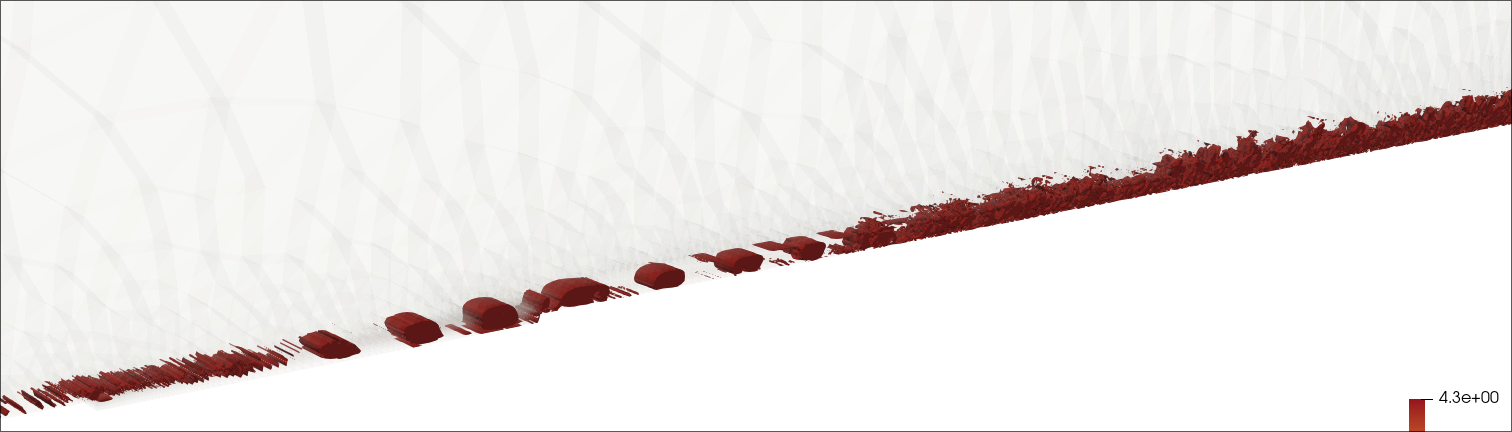
\includegraphics[width=\textwidth]{Images/d1.5w80_trans3.png}
		\end{figure}
\end{frame}
\end{document}
